\documentclass[journal]{vgtc}              


\usepackage{mathptmx}
\usepackage{graphicx}
\usepackage{times}
\usepackage{hyperref}
\usepackage{xcolor}
\usepackage{mdframed}
\usepackage{nomencl}
\makenomenclature
\usepackage{siunitx}
\usepackage{tcolorbox}
\hypersetup{
  pdfauthor = {},
  pdftitle = {},
  pdfsubject = {},
  pdfkeywords = {},
  colorlinks=true,
  linkcolor= black,
  citecolor= black,
  pageanchor=false,
  urlcolor = black,
  plainpages = false,
  linktocpage
}


\onlineid{0}
\vgtccategory{Research}
\vgtcinsertpkg



\title{Measurement Device Independence \\ The Key to Good Communication }

\author{Chris Irish and Jonathan Gough}


\abstract
{
With the every advancing development of quantum computation and its ability to breech current security protocols, new approaches to quantum cryptography must be developed. One such approach is \textit{Measurement Device Independent Quantum Key Distribution}. Up until now, MDIQKD has been largely theoretical. For the first MDIQKD has been experimentally verified by researchers from China. A three user, four node MDIQKD network was achieved within the city of Hefei. A \textcolor{orange}{\textbf{"step in the right direction towards a secure global network"}} says one leading MDIQKD theorist.
}

\keywords{MDIQKD, QKD, BB84}


\CCScatlist{
}

  \teaser{ 
 \centering
 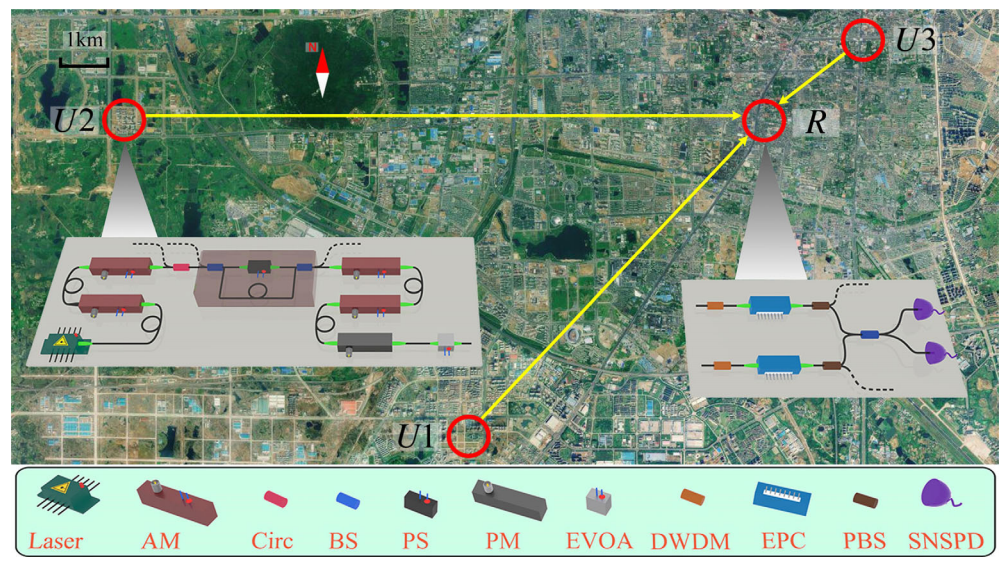
\includegraphics[width=16cm]{map}
  \caption{Birds-eye view of the MDIQKD network topology \cite{PhysRevX.6.011024}.}
  }



\begin{document}


\firstsection{Quantum Cryptography}

\maketitle

At the heart of private communication measures is the secure establishment and distribution of secret \textit{encryption keys}. While the prodigious prime factorisation abilities of quantum computers seem set to make a mockery of our best existing cyber-security measures,
study of quantum communications has simultaneously unearthed a possible lifeline in the form of a new secure key method, whose integrity against eavesdroppers comes with a cast iron guarantee, backed by the laws of quantum physics. At least in theory.

\noindent Meet Eve - she eavesdrops. She also lurks in every theoretical secure communications model, able to instantly recognise any potential weakness, and call on any technology to aid her in its exploitation. A ruthless predator on a single-minded hunt for illicit data, with which to then cause literally any personal damage she can - she's not fussy. Alice and Bob are her nemeses - they're everyone's favourite humble network users, establishing an everyday cryptographic key. They've always been a step ahead, but the second they get complacent Eve will be ready, and she won't settle for less than maximum ruination.



\section{Enter Quantum Key Distribution}

Fortunately, Alice and Bob have a few tricks up their collective sleeve, one of which is \textit{Quantum key distribution} (QKD). The process involves establishing a key from a random bit string, where the bits are transmitted by Alice, each in a basis chosen randomly from a specific set, and received and measured by Bob, each also in a random basis from the set. When the basis choices match, Alice's intended bit state is successfully transferred to Bob.

\noindent Assuming Eve can first find out the bases being used via classical espionage, she may try to intercept Alice's photon, preparing a fake state to send on to Bob, which is known as an \textit{intercept and resend attack}. However, as long as Alice and Bob keep their basis choices secure during the process, Eve has no way to find them out, and subsequently can never be certain of the original value of the bit. The best she can seemingly do is pick basis randomly and send her measured state on to Bob. On top of her 50\% chance to guess the right basis, if she picks wrong she still has a 50\% chance to guess the right bit value, meaning she'll only be wrong a quarter of the time, but it turns out that will be enough.

\noindent After the transmission, Alice and Bob share the sequence of bases they used over a classical phone line. Eve has, of course, bugged the line and hears everything, unbeknownst to our duo but highly suspected. Alice and Bob discard all the results where they used different bases (roughly half), and sacrifice a section of the remaining code by confirming it over the insecure line. By analysing the compromised results, the unavoidable error rate introduced by Eve's tampering can be identified, and with increasing ease the more photons she pilfers.

\noindent However, all is not lost for Eve, as it's a long walk from chalkboard to lab, and she has far sneakier means at her disposal. The real world introduces various problems such as environmental and atmospheric interference, inherent device inaccuracies, creeping alignment errors, and other physical limits to accuracy and scope. And sure enough, down amongst the decay, in with the interference, is Eve, trying to mask her activity behind the systemic noise.



\begin{tcolorbox}
\section*{QKD Basics}

We can create, and transmit, photons with chosen \textit{qubit} states encoded into their polarisation direction. A vertically polarised photon, or $\uparrow$, corresponds to a 1 in our data, while horizontal polarisation, or $\rightarrow$, corresponds to a 0. If we align the emitter with the detector, then when a photon prepared as $\uparrow$, or 1, for instance, reaches the detector, it is measured as $\uparrow$ , or 1, with certainty.

More interestingly, when we tilt either our emitter, or our detector, relative to the other, the probabilities are shifted smoothly from one outcome towards the other. Our measurement will still either be $\uparrow$ or $\rightarrow$ with overall certainty, but with a chance of each outcome. If we tilt our devices at \ang{45} to each other, a photon prepared in either state, $\uparrow$ or $\rightarrow$ , will be measured as $\uparrow$ or $\rightarrow$ with 50/50 chance, and the original information is lost. \textit{BB84} is a common protocol, which uses two different bases, ($\uparrow$, $\rightarrow$) and ($\nwarrow$ , $\nearrow$), that are offset by \ang{45}. This setup employs random number generators to randomise basis choice for both devices, as well as initial bit value. Interference by Eve can be detected by analysing discrepancies in Alice and Bob's results. 

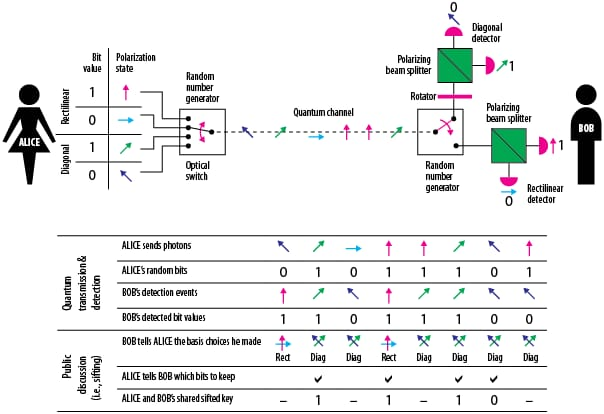
\includegraphics[width=\linewidth]{Box_2}
\textit{Image source: UNS Nice (France), Department of Physics.}

\end{tcolorbox}

 


\section{The Limits of QKD}
\textcolor{black}{"There is no (such) thing as (absolute) security if it always requires some assumptions"}. Dr Lluis Masanes,  A leading researcher on quantum information sciences at UCL has his doubts on standard QKD network security.   

\vspace{0.3cm}

\noindent Previous demonstrations of a \textit{quantum key distribution} networks, such as by the team at Moscow State University\cite{2017QuEle..47..798K} , have been achieved but are still vulnerable to an attack by Eve. Standard QKD networks (also known as prepare and measure QKD networks) have to assume the central relays to be completely trustful. In reality this is extremely unlikely due various security loopholes associated with these networks. One such security loophole is the \textit{detection loophole}. The \textit{detection loophole} is caused by unavoidable losses in the quantum channel and the coupling between photon source and optical fibres. Additionally, losses occur due to the measurement device's finite detection efficiency. This flaw can allow Eve to perform an attack such as an \textit{intercept and resend}.



\section{The Future of QKD}


A MDIQKD network attempts to close the \textit{detection loophole} by removing the standard measurement devices entirely and instead uses a shared  central station to create entanglement-like correlations between Alice and Bob through \textit{Bell-state measurements}(BSM). This approach is based on \textit{time-reversed entanglement based QKD}\cite{PhysRevA.54.2651}. The bell state measurement provides a vital piece of information that when combined with the outgoing information, it allows the network users to work out what information is being sent to them. As only the network user knows his/her outgoing information, even if Eve completely controls the central station she can not gain any information about the cryptographic key. For an MDIQKD network to be successful it requires that the network users have almost perfect state preparation (fully know what their outgoing information is). However this issue is easily addressed as their states can be experimentally verified in a fully protected laboratory environment, outside of Eve's interference.  

QKD networks can be characterised by their \textit{secure key rate}.  The secure key rate gives a measure of how much secure information (measured in bits) is transmitted per second by the network. It is calculated from the network's gain rates, error rates and error correction efficiency. The secure key rate is distinct from the \textit{key rate} which only gives a measure of how much information is transmitted per second by the network. Compared to standard QKD networks, the key rate for an MDIQKD network is relativity low. Under the same experimental parameters a decoy \textit{BB84 system} with a trustful relay can generate a key rate around 1000bps, over 25 times greater than the team achieved in the MDIQKD network. However, what a MDIQKD network lacks in key rate it makes up for with security. Hence, the secure key rate achieved by the team is at least 10 times higher than previous state of the art field tests.

\vspace{0.3cm}

\noindent Prof Alessio Serafini, professor of theoretical physics at UCL reinforced the importance of the team's work for the field of quantum information.

\vspace{0.3cm}

\textcolor{orange}{\textbf{" The theory becomes true when you build a machine with it and Device Independence is very instrumental to this because it tells you these machines can only be quantum, that's in the end what it is.".}}

\section{The Limits of MDI}

Upgrading a network from standard QKD to MDIQKD has not been attempted until now, as there are two main technical challenges that arise. The first being \textit{reference frame calibration}. This refers to the real time alignment of reference frames between network users. In past attempts to achieve \textit{reference frame calibration} researchers have used additional fibre links between users. The results of this is that the demand for fibre links increases quadratically with the number of network users. This is impractical when scaling up to a city sized user populations. A solution was found by the researchers through a \textit{phase feedback scheme}, which allows for a far more manageable linear scaling of fibre links with the number of network users.

\noindent The second technical challenge involves \textit{maintaining indistinguishability} between the network users. In an MDIQKD network any two users can be switched upon request. The new user's signals must be calibrated immediately to disallow the new and old user's signals from mixing. Mixing two users signals would result in the timing, spectrum and polarization mode being indistinguishable between the two users. A solution was developed using a technology called \textit{multi-user HOM interference}. The team believes this technology can find applications in \textit{multi-party entanglement swapping-based quantum communication} and \textit{quantum cloud computing }.


\begin{tcolorbox}
\section*{Typical MDIQKD Process}

1. Alice and Bob both prepare outgoing signals in the four possible polarization states.\\
2. Alice and Bob both send their states to the central relay via optical fibres.\\
3. The central relay performs a bell state measurement that projects the incoming signals into a bell state.\\
4. The relay publicly announces the bell state.\\
5. Alice and Bob then publicly announce their bases but not their associated bits.\\
6. From the relay's bell state, Alice/Bob's bases and knowing their own outgoing bit. Alice/Bob can work out the opposite party's bit that was sent.\\
7. The process is repeated until cryptographic keys are built up.

\end{tcolorbox}


 
\noindent Dr Masanes believes full \textit{Device Independence} provides, in theory, the most secure approach to QKD

\vspace{0.3cm}

\textcolor{orange}{\textbf{"It is easy to say  that it is the most secure framework, but only given that you define the problem in a way that it is possible to do at all".}}

\vspace{0.3cm}

\noindent He believes the problem is in the implementation, as it seems that security loopholes are unavoidable with physical constraints. "Okay, for instance, if my device also broadcasts my secret key it doesn't matter what you do, it's impossible to achieve absolute security". Alternatives exist that attempt to balance theoretical ambitions and practical constraints, such as \textit{Semi-Device Independent} QKD, which requires putting complete trust in some of the devices within your network to boost security overall. The advantage of MDIQKD is that no devices need to be trusted at all. Another issue arises when considering longer distance secure networks as they require additional relays per every few kilometres. "Errors add up in a pretty bad way", says Masanes. Furthermore increasing the number of devices introduces new opportunities for Eve to attack. "What could the adversary do if she had control over the relay? Maybe if she does things cleverly, there is not much that you could do about it".


\section{The Future of MDI}

Scientists are already looking into solutions to these issues, and one new direction they're looking is upwards. "Satellites should be the next step", says Dr Serafini. "If you are able to get above the dense (atmosphere), to almost free space, the signal is less vulnerable to attack", adds Masanes. There are also further potential benefits, such as the presence of existing global satellite networks that could potentially be integrated into QKD networks, and in terms of reducing device requirements, "well, the satellites are very convenient, because otherwise, when the network is big, you need to build lots of optical fibres, for instance". QKD networks are already used in some specific situations within the private sector, such as in secure business transactions. But will developments such as MDIQKD ever see use by the general public? Masanes and Serafini agree that they probably will, but differ over the time frame. Serafini predicts public systems in as little as 5-10 years, whereas Masanes is a little more conservative. "In 15 years (it might be possible) just to say something. Yeah, but I don't think that in 15 years our society will have this (quite yet)".

\vspace{0.3cm}

\noindent It seems likely that before too long, you might find yourself navigating the quantum network, filling in your quantum tax returns. In any case, it looks like Eve's criminal career may soon be over.

\vspace{0.3cm}

\bibliographystyle{unsrt}  
\bibliography{references}

\end{document}
